\documentclass{standalone}
\usepackage{pgfplots}
\pgfplotsset{compat=1.18}

\begin{document}

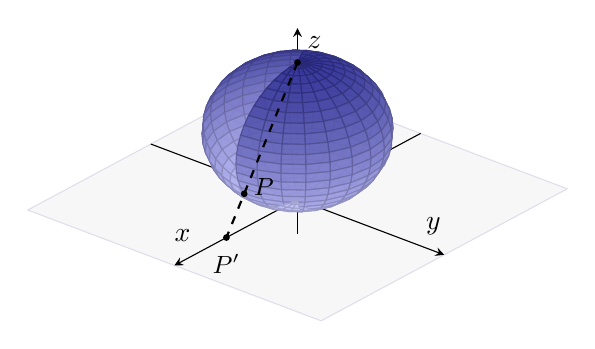
\begin{tikzpicture}[
    declare function={
        sqrt3 = sqrt(3);
    }]
    
\begin{axis}[
    view={130}{40},  % Changed viewpoint (azimuth=120°, elevation=60°)
    axis lines=center,
    xlabel={$x$}, ylabel={$y$}, zlabel={$z$},
    xmin=-2, xmax=2,
    ymin=-2, ymax=2,
    zmin=-0.5, zmax=2.5,  % Adjusted z-range
    ticks=none,
    clip=false,
    colormap={cool}{rgb255=(200,200,255) rgb255=(50,50,150)},
    set layers,  % Enable layer management
]

% First draw the projection plane
\begin{pgfonlayer}{axis background}
\addplot3[
    surf,
    gray!20,
    opacity=0.3,  % More transparent plane
    samples=2,
    domain=-2:2,
    y domain=-2:2,
] {0};
\end{pgfonlayer}

% Then draw the sphere
\addplot3[
    surf,
    opacity=0.9,  % More opaque sphere
    samples=25,
    domain=0:180,
    y domain=0:360,
] (
    {sin(x)*cos(y)},
    {sin(x)*sin(y)},
    {1 + cos(x)}
);

% North pole (projection center)
\addplot3[only marks, mark=*, mark size=1pt] coordinates {(0,0,2)};
% \node at (axis cs:0,0,2.1) [above] {\small North Pole};

% Point P on sphere (theta=120°, phi=0°)
\addplot3[only marks, mark=*, mark size=1pt] 
    coordinates {({sqrt3/2},0,0.5)};
\node at (axis cs:{sqrt3/2},0,0.6) [right] {\small $P$};

% Projected point P'
\addplot3[only marks, mark=*, mark size=1pt] 
    coordinates {({2*sqrt3/3},0,0)};
\node at (axis cs:{2*sqrt3/3},0,-0.1) [below] {\small $P'$};

% Projection line
\addplot3[dashed, thick] coordinates {
    (0,0,2)
    ({sqrt3/2},0,0.5)
    ({2*sqrt3/3},0,0)
};

% Add coordinate system arrows
% \draw[-latex] (axis cs:0,0,0) -- (axis cs:2,0,0) node[below left] {$x$};
% \draw[-latex] (axis cs:0,0,0) -- (axis cs:0,2,0) node[below right] {$y$};
% \draw[-latex] (axis cs:0,0,0) -- (axis cs:0,0,2.5) node[below left] {$z$};

\end{axis}
\end{tikzpicture}

\end{document}